\chapter{Системы нечеткого вывода на основе несинглтонной фаззификации}\label{ch:ch1}

\section{Методы нечеткого вывода}

Предложенная в 1965 году Заде теория нечетких множеств \cite{zadeh1965} позже была использована для построения нечетких систем, которые нашли свое практическое применение в системах автоматизированного управления \cite{mamdani1975}, \cite{Lee1990}, прогнозирования временных последовательностей на зашумленных временных данных \cite{} и распознавания образов \cite{}.

При нечетком выводе с использованием синглтонной фаззификации, входное значение рассматривается как точное значение измеряемой величины, исключающее какую-либо погрешность измерений. Несинглтонная фаззификация позволяет учесть эту погрешность и передать ее вместе с измеренным значением на вход нечеткого вывода. Такой тип систем был подробно изучен в \cite{mendel}.

В отличии от синглтонной фаззификации, использование несинглтонной фаззификации в процедуре вывода имеет экспоненциальну вычислительную сложность при вычислении композиционного правила вывода. Некоторые работы пытаются направлены на обеспечение практической применимости нечетких систем на основе несинглтонной фаззификации \cite{liang}.

Другая трудность в использовании несинглтонной фаззификации состоит в точном моделировании неопределенной во входных значениях. В большинстве случаев применения несинглтонной фаззификации предполагается, что неопределенность во входах одно из общеизвестных распределений, как правило, гауссовое [6] или треугольное. Для корректного определения характера шума во входных значениях может потребоваться проведение отдельного анализа. Также можно внедрить механизм адаптивного моделирования неопределенности в блок несинглтонной фаззификации нечеткой системы, который бы оценивал уровень шума на основе потока входных данных [2].

\section{Несинглтонная фаззификация}



\begin{figure}[ht]
	\centerfloat{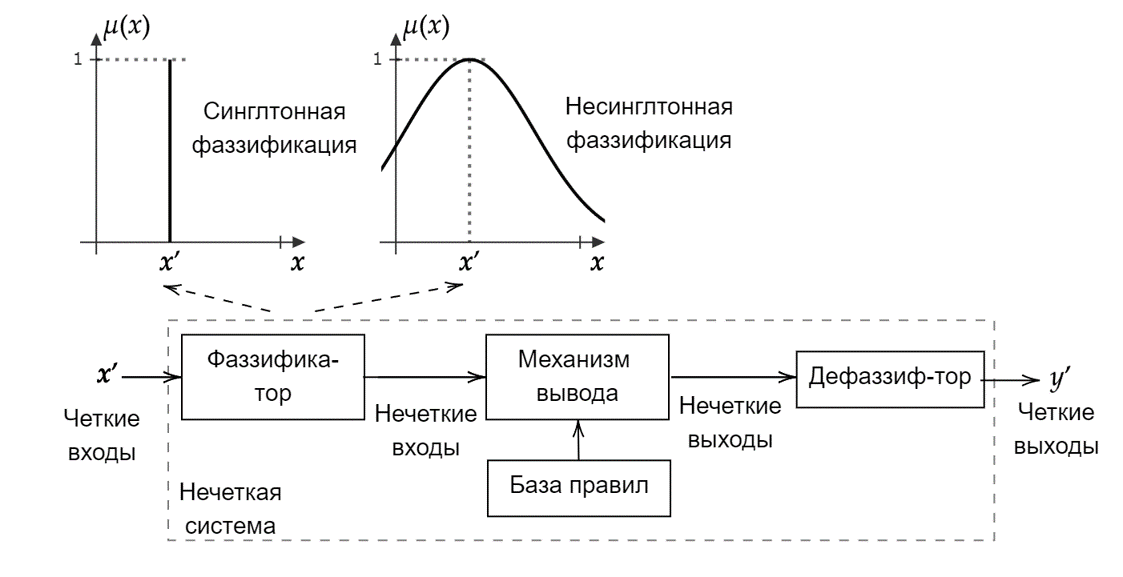
\includegraphics[scale=0.5]{singleton-vs-nonsingleton-fs}}
	\caption{Схема системы нечеткого вывода с использованием синглтонной и несинглтонной фаззификации}\label{fig:singleton-vs-nonsingleton}
\end{figure}

При использовании синглтонной фаззификации поданное на вход нечеткой системы значение интерпретируется как истинное значение измеряемой величины. Однако, в случае .Корректнее описывать значение измеренной величины с учетом компоненты ошибки измерений. В рамках алгебры нечеткой логики подаваемое на вход нечеткой системы значение может быть описано нечетким множеством, степень принадлежноти которого имеет высокие значения как в точке измеренного значения, так и в окрестности оцениваемой величины погрешности этого значения.

Для оценки влияния разницы от использования каждого из двух способов фаззификации на корректность получаемого результата можно для системы логического типа. Мендель в своей книге проводил такое сравнение для систем типа Мамдани. Поскольку в системах типа Мамдани в качестве функции импликации выступает $t$-норма, то разница от применения двух способов фаззификации проявляется в различных максимальных уровнях линии пересечения ф. п. входной посылки и антецедента правила. В зависимости от минимум или произведение. 

Применение композиционного правила вывода sup здесь дает эффект \textit{префильтрации} (или \textit{корректировки}) входного значения. То есть ядра функций принадлежности антецедентов правил выполняют функцию эталонов, а уровень пересечения функции принадлежности для входного значения и ф. п. антецедента правила позволяет интерпретировать входное значение как суперпозицию эталонных значений антецедентов с долями равными этому уровню.

В случае с нечеткой системой логического типа, разница от использования различных способов фаззификации будет проявляться в различных формах выходного нечеткого множества. 

\begin{figure}[ht]
	\begin{minipage}[b][][b]{0.3\linewidth}
		\centering
		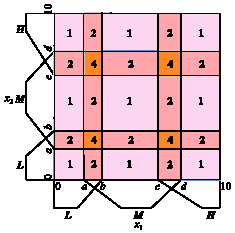
\includegraphics[width=\linewidth, page=1]{ns-fuz-mendel-comparizon-first-order-partition} \\ а
	\end{minipage}
	\hfill
	\begin{minipage}[b][][b]{0.3\linewidth}
		\centering
		\includegraphics[width=\linewidth, page=2]{ns-fuz-mendel-comparizon-first-order-partition} \\ б
	\end{minipage}
	\hfill
	\begin{minipage}[b][][b]{0.3\linewidth}
		\centering
		\includegraphics[width=\linewidth, page=3]{ns-fuz-mendel-comparizon-first-order-partition} \\ в
	\end{minipage}

    \caption{Сравнение }
\end{figure}

В статье [] Мендел также дополнительно иллюстрирует описанное выше с помощью карты разбиений первого и второго порядка на декартовом произведении базовых множеств входных лингвистических переменных. Разбиение первого порядка 

\pgfmathdeclarefunction{gauss}{3}{%
  \pgfmathparse{exp(-((#1-#2)/(2*#3))^2)} % Correct syntax for Gaussian function
}
\pgfmathdeclarefunction{implL}{4}{%
  \pgfmathparse{min(1, 1-#4+gauss(#1, #2, #3))} % Lukasievich
}
\pgfmathdeclarefunction{implR}{4}{%
  \pgfmathparse{min(1, gauss(#1, #2, #3)/#4)} % R
}

\pgfplotsset{
    membership axes/.style={
        width=0.20\textwidth,
        height=0.20\textwidth,
        scale only axis,
        domain=0:1,
        samples=100,
        every axis plot/.append style={smooth},
        axis lines=middle,
        xmin=0, xmax=1,
        ymin=0, ymax=1,
        xticklabel style={font=\tiny, inner sep=1pt, outer sep=0pt},
        yticklabel style={font=\tiny, inner sep=1pt, outer sep=0pt},
    }
}

\begin{figure}[ht]
    \label{fig:ns-width-influence-to-out-mamdani}
    \centering
    \begin{subfigure}[b]{\textwidth}
        \begin{tikzpicture}

        %\begin{scope}[xshift=0cm, yshift=0cm]
            \pgfmathsetmacro{\aZeroMu}{0.55}
            \pgfmathsetmacro{\aFstMu}{0.28}
            \pgfmathsetmacro{\aFstSigma}{0.09}
            \pgfmathsetmacro{\aFstCrossX}{0.55}
            \pgfmathsetmacro{\aFstCrossY}{0.11}
            \pgfmathsetmacro{\aSndMu}{0.5}
            \pgfmathsetmacro{\aSndSigma}{0.08}
            \pgfmathsetmacro{\aSndCrossX}{0.55}
            \pgfmathsetmacro{\aSndCrossY}{0.91}
            \pgfmathsetmacro{\aTrdMu}{0.89}
            \pgfmathsetmacro{\aTrdSigma}{0.2}
            \pgfmathsetmacro{\aTrdCrossX}{0.55}
            \pgfmathsetmacro{\aTrdCrossY}{0.49}
            \pgfmathsetmacro{\bFstMu}{0.2}
            \pgfmathsetmacro{\bFstSigma}{0.12}
            \pgfmathsetmacro{\bSndMu}{0.5}
            \pgfmathsetmacro{\bSndSigma}{0.1}
            \pgfmathsetmacro{\bTrdMu}{0.8}
            \pgfmathsetmacro{\bTrdSigma}{0.1}

            % First function
            \begin{axis}[
                membership axes,
                name=plot1,
                at={(0,0)},
                xlabel={$x_1$},
                ylabel={$\mu$},
                xlabel style={font=\footnotesize, at=(current axis.south), anchor=north, yshift=-10pt},
                ylabel style={font=\footnotesize, at=(current axis.west), anchor=east, xshift=-10pt},
            ]
                \addplot[blue, name path=A0] coordinates {(\aZeroMu, 0) (\aZeroMu, 1)};
                \addplot[black, name path=A1] {gauss(\x, \aFstMu, \aFstSigma)};
                \addplot[only marks, mark=*, mark size=2pt, purple!50] coordinates {(\aFstCrossX,\aFstCrossY)};
                \coordinate (fire11) at (axis cs:\aFstCrossX,\aFstCrossY); % USE axis cs
            \end{axis}
            % Second function
            \begin{axis}[
                membership axes,
                name=plot2,
                at={(0.25\textwidth,0)},
                xlabel={$x_2$},
                ylabel={$\mu$},
                xlabel style={font=\footnotesize, at=(current axis.south), anchor=north, yshift=-10pt},
                ylabel style={font=\footnotesize, at=(current axis.west), anchor=east, xshift=-10pt},
            ]
                \addplot[blue, name path=A0] coordinates {(\aZeroMu, 0) (\aZeroMu, 1)};
                \addplot[black, name path=A1] {gauss(\x, \aSndMu, \aSndSigma)};
                \addplot[only marks, mark=*, mark size=2pt, lime] coordinates {(\aSndCrossX,\aSndCrossY)};
                \coordinate (fire12) at (axis cs:\aSndCrossX,\aSndCrossY); % Use axis cs
            \end{axis}
            % Third function
            \begin{axis}[
                membership axes,
                name=plot3,
                at={(0.5\textwidth,0)},
                xlabel={$x_3$},
                ylabel={$\mu$},
                xlabel style={font=\footnotesize, at=(current axis.south), anchor=north, yshift=-10pt},
                ylabel style={font=\footnotesize, at=(current axis.west), anchor=east, xshift=-10pt},
            ]
                \addplot[blue, name path=A0] coordinates {(\aZeroMu, 0) (\aZeroMu, 1)};
                \addplot[black, name path=A1] {gauss(\x, \aTrdMu, \aTrdSigma)};
                \addplot[only marks, mark=*, mark size=2pt, cyan!50] coordinates {(\aTrdCrossX,\aTrdCrossY)};
                \coordinate (fire13) at (axis cs:\aTrdCrossX,\aTrdCrossY); % Use axis cs
            \end{axis}
            % Fourth function
            \begin{axis}[
                membership axes,
                name=plot4,
                at={(0.75\textwidth,0)},
                xlabel={$y$},
                ylabel={$\mu_{B'}(y)$},
                xlabel style={font=\footnotesize, at=(current axis.south), anchor=north, yshift=-10pt},
                ylabel style={font=\footnotesize, at=(current axis.above origin), anchor=south},
            ]
                \addplot [purple!50] {min(\aFstCrossY, gauss(\x, \bFstMu, \bFstSigma))};
                \addplot [lime] {min(\aSndCrossY, gauss(\x, \bSndMu, \bSndSigma))};
                \addplot [cyan!50] {min(\aTrdCrossY, gauss(\x, \bTrdMu, \bTrdSigma))};
                \addplot[fill=orange!30, orange] {max(min(\aFstCrossY, gauss(\x, \bFstMu, \bFstSigma)), min(\aSndCrossY, gauss(\x, \bSndMu, \bSndSigma)), min(\aTrdCrossY, gauss(\x, \bTrdMu, \bTrdSigma)))} \closedcycle;
                \coordinate (out11) at (axis cs:0.0,\aFstCrossY); % Use axis cs
                \coordinate (out12) at (axis cs:0.0,\aSndCrossY); % Use axis cs
                \coordinate (out13) at (axis cs:0.0,\aTrdCrossY); % Use axis cs
            \end{axis}

            % Connect coordinates using defined coordinate names
            \draw [purple!50, dashed, thick] (fire11) -- (out11);
            \draw [lime, dashed, thick] (fire12) -- (out12);
            \draw [cyan!50, dashed, thick] (fire13) -- (out13);

            % \node {\sigma=\aZeroSigma};
            \node[left, xshift=-1.2cm, font=\footnotesize, rotate=90, anchor=center] at (plot1.west) {$\sigma_{A'}=0$};
        \end{tikzpicture}
	\end{subfigure}
	
	%%
	\vspace{0.1cm}
	%%
	
	\begin{subfigure}[b]{\textwidth}
        \begin{tikzpicture}

        %\begin{scope}[xshift=0cm, yshift=0cm]
            \pgfmathsetmacro{\aZeroMu}{0.55}
            \pgfmathsetmacro{\aZeroSigma}{0.01}
            \pgfmathsetmacro{\aFstMu}{0.28}
            \pgfmathsetmacro{\aFstSigma}{0.09}
            \pgfmathsetmacro{\aFstCrossX}{0.515}
            \pgfmathsetmacro{\aFstCrossY}{0.185}
            \pgfmathsetmacro{\aSndMu}{0.5}
            \pgfmathsetmacro{\aSndSigma}{0.08}
            \pgfmathsetmacro{\aSndCrossX}{0.56}
            \pgfmathsetmacro{\aSndCrossY}{0.88}
            \pgfmathsetmacro{\aTrdMu}{0.89}
            \pgfmathsetmacro{\aTrdSigma}{0.2}
            \pgfmathsetmacro{\aTrdCrossX}{0.57}
            \pgfmathsetmacro{\aTrdCrossY}{0.53}
            \pgfmathsetmacro{\bFstMu}{0.2}
            \pgfmathsetmacro{\bFstSigma}{0.12}
            \pgfmathsetmacro{\bSndMu}{0.5}
            \pgfmathsetmacro{\bSndSigma}{0.1}
            \pgfmathsetmacro{\bTrdMu}{0.8}
            \pgfmathsetmacro{\bTrdSigma}{0.1}

            % First function
            \begin{axis}[
                membership axes,
                name=plot1,
                at={(0,0)},
                xlabel={$x_1$},
                ylabel={$\mu$},
                xlabel style={},
                xlabel style={font=\footnotesize, at=(current axis.south), anchor=north, yshift=-10pt},
                ylabel style={font=\footnotesize, at=(current axis.west), anchor=east, xshift=-10pt},
            ]
                \addplot[blue, name path=A0] {gauss(\x, \aZeroMu, \aZeroSigma)};
                \addplot[black, name path=A1] {gauss(\x, \aFstMu, \aFstSigma)};
                \addplot[fill=purple!50, draw=none] {min(gauss(\x, \aZeroMu, \aZeroSigma), gauss(\x, \aFstMu, \aFstSigma))} \closedcycle;
                \coordinate (fire11) at (axis cs:\aFstCrossX,\aFstCrossY); % USE axis cs
            \end{axis}
            % Second function
            \begin{axis}[
                membership axes,
                name=plot2,
                at={(0.25\textwidth,0)},
                xlabel={$x_2$},
                ylabel={$\mu$},
                xlabel style={font=\footnotesize, at=(current axis.south), anchor=north, yshift=-10pt},
                ylabel style={font=\footnotesize, at=(current axis.west), anchor=east, xshift=-10pt},
            ]
                \addplot[blue, name path=A0] {gauss(\x, \aZeroMu, \aZeroSigma)};
                \addplot[black, name path=A1] {gauss(\x, \aSndMu, \aSndSigma)};
                \addplot[fill=lime, draw=none] {min(gauss(\x, \aZeroMu, \aZeroSigma), gauss(\x, \aSndMu, \aSndSigma))} \closedcycle;
                \coordinate (fire12) at (axis cs:\aSndCrossX,\aSndCrossY); % Use axis cs
            \end{axis}
            % Third function
            \begin{axis}[
                membership axes,
                name=plot3,
                at={(0.5\textwidth,0)},
                xlabel={$x_3$},
                ylabel={$\mu$},
                xlabel style={font=\footnotesize, at=(current axis.south), anchor=north, yshift=-10pt},
                ylabel style={font=\footnotesize, at=(current axis.west), anchor=east, xshift=-10pt},
            ]
                \addplot[blue, name path=A0] {gauss(\x, \aZeroMu, \aZeroSigma)};
                \addplot[black, name path=A1] {gauss(\x, \aTrdMu, \aTrdSigma)};
                \addplot[fill=cyan!50, draw=none] {min(gauss(\x, \aZeroMu, \aZeroSigma), gauss(\x, \aTrdMu, \aTrdSigma))} \closedcycle;
                \coordinate (fire13) at (axis cs:\aTrdCrossX,\aTrdCrossY); % Use axis cs
            \end{axis}
            % Fourth function
            \begin{axis}[
                membership axes,
                name=plot4,
                at={(0.75\textwidth,0)},
                xlabel={$y$},
                ylabel={$\mu_{B'}(y)$},
                xlabel style={font=\footnotesize, at=(current axis.south), anchor=north, yshift=-10pt},
                ylabel style={font=\footnotesize, at=(current axis.above origin), anchor=south},
            ]
                \addplot [purple!50] {min(\aFstCrossY, gauss(\x, \bFstMu, \bFstSigma))};
                \addplot [lime] {min(\aSndCrossY, gauss(\x, \bSndMu, \bSndSigma))};
                \addplot [cyan!50] {min(\aTrdCrossY, gauss(\x, \bTrdMu, \bTrdSigma))};
                \addplot[fill=orange!30, orange] {max(min(\aFstCrossY, gauss(\x, \bFstMu, \bFstSigma)), min(\aSndCrossY, gauss(\x, \bSndMu, \bSndSigma)), min(\aTrdCrossY, gauss(\x, \bTrdMu, \bTrdSigma)))} \closedcycle;
                \coordinate (out11) at (axis cs:0.0,\aFstCrossY); % Use axis cs
                \coordinate (out12) at (axis cs:0.0,\aSndCrossY); % Use axis cs
                \coordinate (out13) at (axis cs:0.0,\aTrdCrossY); % Use axis cs
            \end{axis}

            % Connect coordinates using defined coordinate names
            \draw [purple!50, dashed, thick] (fire11) -- (out11);
            \draw [lime, dashed, thick] (fire12) -- (out12);
            \draw [cyan!50, dashed, thick] (fire13) -- (out13);

            % \node {\sigma=\aZeroSigma};
            \node[left, xshift=-1.2cm, font=\footnotesize, rotate=90, anchor=center] at (plot1.west) {$\sigma_{A'}=\aZeroSigma$};
        \end{tikzpicture}
	\end{subfigure}
	
	%%
	\vspace{0.1cm}
	%%
	
	\begin{subfigure}[b]{\textwidth}
          \begin{tikzpicture}
            \pgfmathsetmacro{\aZeroMu}{0.55}
            \pgfmathsetmacro{\aZeroSigma}{0.05}
            \pgfmathsetmacro{\aFstMu}{0.28}
            \pgfmathsetmacro{\aFstSigma}{0.09}
            \pgfmathsetmacro{\aFstCrossX}{0.49}
            \pgfmathsetmacro{\aFstCrossY}{0.4}
            \pgfmathsetmacro{\aSndMu}{0.5}
            \pgfmathsetmacro{\aSndSigma}{0.08}
            \pgfmathsetmacro{\aSndCrossX}{0.53}
            \pgfmathsetmacro{\aSndCrossY}{0.97}
            \pgfmathsetmacro{\aTrdMu}{0.89}
            \pgfmathsetmacro{\aTrdSigma}{0.2}
            \pgfmathsetmacro{\aTrdCrossX}{0.6}
            \pgfmathsetmacro{\aTrdCrossY}{0.61}
            \pgfmathsetmacro{\bFstMu}{0.2}
            \pgfmathsetmacro{\bFstSigma}{0.12}
            \pgfmathsetmacro{\bSndMu}{0.5}
            \pgfmathsetmacro{\bSndSigma}{0.1}
            \pgfmathsetmacro{\bTrdMu}{0.8}
            \pgfmathsetmacro{\bTrdSigma}{0.1}

            % First function
            \begin{axis}[
                membership axes,
                name=plot1,
                at={(0,0)},
                xlabel={$x_1$},
                ylabel={$\mu$},
                xlabel style={font=\footnotesize, at=(current axis.south), anchor=north, yshift=-10pt},
                ylabel style={font=\footnotesize, at=(current axis.west), anchor=east, xshift=-10pt},
            ]
                \addplot[blue, name path=A0] {gauss(\x, \aZeroMu, \aZeroSigma)};
                \addplot[black, name path=A1] {gauss(\x, \aFstMu, \aFstSigma)};
                \addplot[fill=purple!50, draw=none] {min(gauss(\x, \aZeroMu, \aZeroSigma), gauss(\x, \aFstMu, \aFstSigma))} \closedcycle;
                \coordinate (fire11) at (axis cs:\aFstCrossX,\aFstCrossY); % USE axis cs
            \end{axis}
            % Second function
            \begin{axis}[
                membership axes,
                name=plot2,
                at={(0.25\textwidth,0)},
                xlabel={$x_2$},
                ylabel={$\mu$},
                xlabel style={font=\footnotesize, at=(current axis.south), anchor=north, yshift=-10pt},
                ylabel style={font=\footnotesize, at=(current axis.west), anchor=east, xshift=-10pt},
            ]
                \addplot[blue, name path=A0] {gauss(\x, \aZeroMu, \aZeroSigma)};
                \addplot[black, name path=A1] {gauss(\x, \aSndMu, \aSndSigma)};
                \addplot[fill=lime, draw=none] {min(gauss(\x, \aZeroMu, \aZeroSigma), gauss(\x, \aSndMu, \aSndSigma))} \closedcycle;
                \coordinate (fire12) at (axis cs:\aSndCrossX,\aSndCrossY); % Use axis cs
            \end{axis}
            % Third function
            \begin{axis}[
                membership axes,
                name=plot2,
                at={(0.5\textwidth,0)},
                xlabel={$x_3$},
                ylabel={$\mu$},
                xlabel style={font=\footnotesize, at=(current axis.south), anchor=north, yshift=-10pt},
                ylabel style={font=\footnotesize, at=(current axis.west), anchor=east, xshift=-10pt},
            ]
                \addplot[blue, name path=A0] {gauss(\x, \aZeroMu, \aZeroSigma)};
                \addplot[black, name path=A1] {gauss(\x, \aTrdMu, \aTrdSigma)};
                \addplot[fill=cyan!50, draw=none] {min(gauss(\x, \aZeroMu, \aZeroSigma), gauss(\x, \aTrdMu, \aTrdSigma))} \closedcycle;
                \coordinate (fire13) at (axis cs:\aTrdCrossX,\aTrdCrossY); % Use axis cs
            \end{axis}
            % Fourth function
            \begin{axis}[
                membership axes,
                name=plot4,
                at={(0.75\textwidth,0)},
                xlabel={$y$},
                ylabel={$\mu_{B'}(y)$},
                xlabel style={font=\footnotesize, at=(current axis.south), anchor=north, yshift=-10pt},
                ylabel style={font=\footnotesize, at=(current axis.above origin), anchor=south},
            ]
                \addplot [purple!50] {min(\aFstCrossY, gauss(\x, \bFstMu, \bFstSigma))};
                \addplot [lime] {min(\aSndCrossY, gauss(\x, \bSndMu, \bSndSigma))};
                \addplot [cyan!50] {min(\aTrdCrossY, gauss(\x, \bTrdMu, \bTrdSigma))};
                \addplot[fill=orange!30, orange] {max(min(\aFstCrossY, gauss(\x, \bFstMu, \bFstSigma)), min(\aSndCrossY, gauss(\x, \bSndMu, \bSndSigma)), min(\aTrdCrossY, gauss(\x, \bTrdMu, \bTrdSigma)))} \closedcycle;
                \coordinate (out11) at (axis cs:0.0,\aFstCrossY); % Use axis cs
                \coordinate (out12) at (axis cs:0.0,\aSndCrossY); % Use axis cs
                \coordinate (out13) at (axis cs:0.0,\aTrdCrossY); % Use axis cs
            \end{axis}

            % Connect coordinates using defined coordinate names
            \draw [purple!50, dashed, thick] (fire11) -- (out11);
            \draw [lime, dashed, thick] (fire12) -- (out12);
            \draw [cyan!50, dashed, thick] (fire13) -- (out13);

            % \node {\sigma=\aZeroSigma};
            \node[left, xshift=-1.2cm, font=\footnotesize, rotate=90, anchor=center] at (plot1.west) {$\sigma_{A'}=\aZeroSigma$};
        \end{tikzpicture}
    \end{subfigure}
    \caption{Сравнение формы функции принадлежности для подхода Мамдани}
\end{figure}

Показанная на этих схемах динамика более ясно раскрыта на рисунке \cref{fig:ns-width-influence-to-out-mamdani} для различных значениях среднеквадратичного отклонения в гауссовой ф. п. входного значения на примере агрегации выходной ф. п. нечеткой системы с тремя правилами в базе правил. Видно, что при переходе от синглтонной фаззификации к несинглтонной и при дальнейшем увеличении ширины среднеквадратичного отклонения ф. п. входного нечеткого множества, повышается уровень срабатывания первого правила, и, как следствие использования импликации Мамдани, уровень задействования ф. .п выходного нечеткого множества этого правила в результирующей агрегации. Кроме того, можно пронаблюдать, упомянутый ранее, эффект префильтрации входного значения антецедентом третьего правила.



\begin{figure}[ht]
    \label{fig:ns-width-influence-to-out-logical}
    \centering
    \begin{subfigure}[b]{\textwidth}
        \begin{tikzpicture}

        %\begin{scope}[xshift=0cm, yshift=0cm]
            \pgfmathsetmacro{\aZeroMu}{0.55}
            \pgfmathsetmacro{\aFstMu}{0.28}
            \pgfmathsetmacro{\aFstSigma}{0.09}
            \pgfmathsetmacro{\aFstCrossX}{0.55}
            \pgfmathsetmacro{\aFstCrossY}{0.11}
            \pgfmathsetmacro{\aSndMu}{0.5}
            \pgfmathsetmacro{\aSndSigma}{0.08}
            \pgfmathsetmacro{\aSndCrossX}{0.55}
            \pgfmathsetmacro{\aSndCrossY}{0.91}
            \pgfmathsetmacro{\aTrdMu}{0.89}
            \pgfmathsetmacro{\aTrdSigma}{0.2}
            \pgfmathsetmacro{\aTrdCrossX}{0.55}
            \pgfmathsetmacro{\aTrdCrossY}{0.49}
            \pgfmathsetmacro{\bFstMu}{0.2}
            \pgfmathsetmacro{\bFstSigma}{0.12}
            \pgfmathsetmacro{\bSndMu}{0.5}
            \pgfmathsetmacro{\bSndSigma}{0.1}
            \pgfmathsetmacro{\bTrdMu}{0.8}
            \pgfmathsetmacro{\bTrdSigma}{0.1}

            % First function
            \begin{axis}[
                membership axes,
                name=plot1,
                at={(0,0)},
                xlabel={$x_1$},
                ylabel={$\mu$},
                xlabel style={font=\footnotesize, at=(current axis.south), anchor=north},
                ylabel style={font=\footnotesize, at=(current axis.west), anchor=east, xshift=-10pt},
                y dir=reverse,
                % axis x line=top,
                xticklabel pos=upper,
                xticklabel style={yshift=13pt}
            ]
                \addplot[blue, name path=A0] coordinates {(\aZeroMu, 0) (\aZeroMu, 1)};
                \addplot[black, name path=A1] {gauss(\x, \aFstMu, \aFstSigma)};
                \addplot[only marks, mark=*, mark size=2pt, purple!50] coordinates {(\aFstCrossX,\aFstCrossY)};
                \coordinate (fire11) at (axis cs:\aFstCrossX,\aFstCrossY); % USE axis cs
            \end{axis}
            % Second function
            \begin{axis}[
                membership axes,
                name=plot2,
                at={(0.25\textwidth,0)},
                xlabel={$x_2$},
                ylabel={$\mu$},
                xlabel style={font=\footnotesize, at=(current axis.south), anchor=north},
                ylabel style={font=\footnotesize, at=(current axis.west), anchor=east, xshift=-10pt},
                y dir=reverse,
                % axis x line=top,
                xticklabel pos=upper,
                xticklabel style={yshift=13pt}
            ]
                \addplot[blue, name path=A0] coordinates {(\aZeroMu, 0) (\aZeroMu, 1)};
                \addplot[black, name path=A1] {gauss(\x, \aSndMu, \aSndSigma)};
                \addplot[only marks, mark=*, mark size=2pt, lime] coordinates {(\aSndCrossX,\aSndCrossY)};
                \coordinate (fire12) at (axis cs:\aSndCrossX,\aSndCrossY); % Use axis cs
            \end{axis}
            % Third function
            \begin{axis}[
                membership axes,
                name=plot3,
                at={(0.5\textwidth,0)},
                xlabel={$x_3$},
                ylabel={$\mu$},
                xlabel style={font=\footnotesize, at=(current axis.south), anchor=north},
                ylabel style={font=\footnotesize, at=(current axis.west), anchor=east, xshift=-10pt},
                y dir=reverse,
                % axis x line=top,
                xticklabel pos=upper,
                xticklabel style={yshift=13pt}
            ]
                \addplot[blue, name path=A0] coordinates {(\aZeroMu, 0) (\aZeroMu, 1)};
                \addplot[black, name path=A1] {gauss(\x, \aTrdMu, \aTrdSigma)};
                \addplot[only marks, mark=*, mark size=2pt, cyan!50] coordinates {(\aTrdCrossX,\aTrdCrossY)};
                \coordinate (fire13) at (axis cs:\aTrdCrossX,\aTrdCrossY); % Use axis cs
            \end{axis}
            % Fourth function
            \begin{axis}[
                membership axes,
                name=plot4,
                at={(0.75\textwidth,0)},
                xlabel={$y$},
                ylabel={$\mu_{B'}(y)$},
                xlabel style={font=\footnotesize, at=(current axis.south), anchor=north, yshift=-10pt},
                ylabel style={font=\footnotesize, at=(current axis.above origin), anchor=south},
            ]
                \addplot [purple!50] {implL(\x, \bFstMu, \bFstSigma, \aFstCrossY)};
                \addplot [lime] {implL(\x, \bSndMu, \bSndSigma, \aSndCrossY)};
                \addplot [cyan!50] {implL(\x, \bTrdMu, \bTrdSigma, \aTrdCrossY)};
                \addplot[fill=orange!30, orange] {min(implL(\x, \bFstMu, \bFstSigma, \aFstCrossY), implL(\x, \bSndMu, \bSndSigma, \aSndCrossY), implL(\x, \bTrdMu, \bTrdSigma, \aTrdCrossY))} \closedcycle;
                \coordinate (out11) at (axis cs:0.0,1-\aFstCrossY); % Use axis cs
                \coordinate (out12) at (axis cs:0.0,1-\aSndCrossY); % Use axis cs
                \coordinate (out13) at (axis cs:0.0,1-\aTrdCrossY); % Use axis cs
            \end{axis}

            % Connect coordinates using defined coordinate names
            \draw [purple!50, dashed, thick] (fire11) -- (out11);
            \draw [lime, dashed, thick] (fire12) -- (out12);
            \draw [cyan!50, dashed, thick] (fire13) -- (out13);

            % \node {\sigma=\aZeroSigma};
            \node[left, xshift=-1.2cm, font=\footnotesize, rotate=90, anchor=center] at (plot1.west) {$\sigma_{A'}=0$};
        \end{tikzpicture}
	\end{subfigure}
	
	%%
	\vspace{0.1cm}
	%%
	
	\begin{subfigure}[b]{\textwidth}
        \begin{tikzpicture}

        %\begin{scope}[xshift=0cm, yshift=0cm]
            \pgfmathsetmacro{\aZeroMu}{0.55}
            \pgfmathsetmacro{\aZeroSigma}{0.01}
            \pgfmathsetmacro{\aFstMu}{0.28}
            \pgfmathsetmacro{\aFstSigma}{0.09}
            \pgfmathsetmacro{\aFstCrossX}{0.515}
            \pgfmathsetmacro{\aFstCrossY}{0.185}
            \pgfmathsetmacro{\aSndMu}{0.5}
            \pgfmathsetmacro{\aSndSigma}{0.08}
            \pgfmathsetmacro{\aSndCrossX}{0.56}
            \pgfmathsetmacro{\aSndCrossY}{0.88}
            \pgfmathsetmacro{\aTrdMu}{0.89}
            \pgfmathsetmacro{\aTrdSigma}{0.2}
            \pgfmathsetmacro{\aTrdCrossX}{0.57}
            \pgfmathsetmacro{\aTrdCrossY}{0.53}
            \pgfmathsetmacro{\bFstMu}{0.2}
            \pgfmathsetmacro{\bFstSigma}{0.12}
            \pgfmathsetmacro{\bSndMu}{0.5}
            \pgfmathsetmacro{\bSndSigma}{0.1}
            \pgfmathsetmacro{\bTrdMu}{0.8}
            \pgfmathsetmacro{\bTrdSigma}{0.1}

            % First function
            \begin{axis}[
                membership axes,
                name=plot1,
                at={(0,0)},
                xlabel={$x_1$},
                ylabel={$\mu$},
                xlabel style={font=\footnotesize, at=(current axis.south), anchor=north},
                ylabel style={font=\footnotesize, at=(current axis.west), anchor=east, xshift=-10pt},
                y dir=reverse,
                % axis x line=top,
                xticklabel pos=upper,
                xticklabel style={yshift=13pt}
            ]
                \addplot[blue, name path=A0] {gauss(\x, \aZeroMu, \aZeroSigma)};
                \addplot[black, name path=A1] {gauss(\x, \aFstMu, \aFstSigma)};
                \addplot[fill=purple!50, draw=none] {min(gauss(\x, \aZeroMu, \aZeroSigma), gauss(\x, \aFstMu, \aFstSigma))} \closedcycle;
                \coordinate (fire11) at (axis cs:\aFstCrossX,\aFstCrossY); % USE axis cs
            \end{axis}
            % Second function
            \begin{axis}[
                membership axes,
                name=plot2,
                at={(0.25\textwidth,0)},
                xlabel={$x_2$},
                ylabel={$\mu$},
                xlabel style={font=\footnotesize, at=(current axis.south), anchor=north},
                ylabel style={font=\footnotesize, at=(current axis.west), anchor=east, xshift=-10pt},
                y dir=reverse,
                % axis x line=top,
                xticklabel pos=upper,
                xticklabel style={yshift=13pt}
            ]
                \addplot[blue, name path=A0] {gauss(\x, \aZeroMu, \aZeroSigma)};
                \addplot[black, name path=A1] {gauss(\x, \aSndMu, \aSndSigma)};
                \addplot[fill=lime, draw=none] {min(gauss(\x, \aZeroMu, \aZeroSigma), gauss(\x, \aSndMu, \aSndSigma))} \closedcycle;
                \coordinate (fire12) at (axis cs:\aSndCrossX,\aSndCrossY); % Use axis cs
            \end{axis}
            % Third function
            \begin{axis}[
                membership axes,
                name=plot3,
                at={(0.5\textwidth,0)},
                xlabel={$x_3$},
                ylabel={$\mu$},
                xlabel style={font=\footnotesize, at=(current axis.south), anchor=north},
                ylabel style={font=\footnotesize, at=(current axis.west), anchor=east, xshift=-10pt},
                y dir=reverse,
                % axis x line=top,
                xticklabel pos=upper,
                xticklabel style={yshift=13pt}
            ]
                \addplot[blue, name path=A0] {gauss(\x, \aZeroMu, \aZeroSigma)};
                \addplot[black, name path=A1] {gauss(\x, \aTrdMu, \aTrdSigma)};
                \addplot[fill=cyan!50, draw=none] {min(gauss(\x, \aZeroMu, \aZeroSigma), gauss(\x, \aTrdMu, \aTrdSigma))} \closedcycle;
                \coordinate (fire13) at (axis cs:\aTrdCrossX,\aTrdCrossY); % Use axis cs
            \end{axis}
            % Fourth function
            \begin{axis}[
                membership axes,
                name=plot4,
                at={(0.75\textwidth,0)},
                xlabel={$y$},
                ylabel={$\mu_{B'}(y)$},
                xlabel style={font=\footnotesize, at=(current axis.south), anchor=north, yshift=-10pt},
                ylabel style={font=\footnotesize, at=(current axis.above origin), anchor=south},
            ]
                \addplot [purple!50] {implL(\x, \bFstMu, \bFstSigma, \aFstCrossY)};
                \addplot [lime] {implL(\x, \bSndMu, \bSndSigma, \aSndCrossY)};
                \addplot [cyan!50] {implL(\x, \bTrdMu, \bTrdSigma, \aTrdCrossY)};
                \addplot[fill=orange!30, orange] {min(implL(\x, \bFstMu, \bFstSigma, \aFstCrossY), implL(\x, \bSndMu, \bSndSigma, \aSndCrossY), implL(\x, \bTrdMu, \bTrdSigma, \aTrdCrossY))} \closedcycle;
                \coordinate (out11) at (axis cs:0.0,1-\aFstCrossY); % Use axis cs
                \coordinate (out12) at (axis cs:0.0,1-\aSndCrossY); % Use axis cs
                \coordinate (out13) at (axis cs:0.0,1-\aTrdCrossY); % Use axis cs
            \end{axis}

            % Connect coordinates using defined coordinate names
            \draw [purple!50, dashed, thick] (fire11) -- (out11);
            \draw [lime, dashed, thick] (fire12) -- (out12);
            \draw [cyan!50, dashed, thick] (fire13) -- (out13);

            % \node {\sigma=\aZeroSigma};
            \node[left, xshift=-1.2cm, font=\footnotesize, rotate=90, anchor=center] at (plot1.west) {$\sigma_{A'}=\aZeroSigma$};
        \end{tikzpicture}
	\end{subfigure}
	
	%%
	\vspace{0.1cm}
	%%
	
	\begin{subfigure}[b]{\textwidth}
          \begin{tikzpicture}
            \pgfmathsetmacro{\aZeroMu}{0.55}
            \pgfmathsetmacro{\aZeroSigma}{0.05}
            \pgfmathsetmacro{\aFstMu}{0.28}
            \pgfmathsetmacro{\aFstSigma}{0.09}
            \pgfmathsetmacro{\aFstCrossX}{0.49}
            \pgfmathsetmacro{\aFstCrossY}{0.4}
            \pgfmathsetmacro{\aSndMu}{0.5}
            \pgfmathsetmacro{\aSndSigma}{0.08}
            \pgfmathsetmacro{\aSndCrossX}{0.53}
            \pgfmathsetmacro{\aSndCrossY}{0.97}
            \pgfmathsetmacro{\aTrdMu}{0.89}
            \pgfmathsetmacro{\aTrdSigma}{0.2}
            \pgfmathsetmacro{\aTrdCrossX}{0.6}
            \pgfmathsetmacro{\aTrdCrossY}{0.61}
            \pgfmathsetmacro{\bFstMu}{0.2}
            \pgfmathsetmacro{\bFstSigma}{0.12}
            \pgfmathsetmacro{\bSndMu}{0.5}
            \pgfmathsetmacro{\bSndSigma}{0.1}
            \pgfmathsetmacro{\bTrdMu}{0.8}
            \pgfmathsetmacro{\bTrdSigma}{0.1}

            % First function
            \begin{axis}[
                membership axes,
                name=plot1,
                at={(0,0)},
                xlabel={$x_1$},
                ylabel={$\mu$},
                xlabel style={font=\footnotesize, at=(current axis.south), anchor=north},
                ylabel style={font=\footnotesize, at=(current axis.west), anchor=east, xshift=-10pt},
                y dir=reverse,
                % axis x line=top,
                xticklabel pos=upper,
                xticklabel style={yshift=13pt}
            ]
                \addplot[blue, name path=A0] {gauss(\x, \aZeroMu, \aZeroSigma)};
                \addplot[black, name path=A1] {gauss(\x, \aFstMu, \aFstSigma)};
                \addplot[fill=purple!50, draw=none] {min(gauss(\x, \aZeroMu, \aZeroSigma), gauss(\x, \aFstMu, \aFstSigma))} \closedcycle;
                \coordinate (fire11) at (axis cs:\aFstCrossX,\aFstCrossY); % USE axis cs
            \end{axis}
            % Second function
            \begin{axis}[
                membership axes,
                name=plot2,
                at={(0.25\textwidth,0)},
                xlabel={$x_2$},
                ylabel={$\mu$},
                xlabel style={font=\footnotesize, at=(current axis.south), anchor=north},
                ylabel style={font=\footnotesize, at=(current axis.west), anchor=east, xshift=-10pt},
                y dir=reverse,
                % axis x line=top,
                xticklabel pos=upper,
                xticklabel style={yshift=13pt}
            ]
                \addplot[blue, name path=A0] {gauss(\x, \aZeroMu, \aZeroSigma)};
                \addplot[black, name path=A1] {gauss(\x, \aSndMu, \aSndSigma)};
                \addplot[fill=lime, draw=none] {min(gauss(\x, \aZeroMu, \aZeroSigma), gauss(\x, \aSndMu, \aSndSigma))} \closedcycle;
                \coordinate (fire12) at (axis cs:\aSndCrossX,\aSndCrossY); % Use axis cs
            \end{axis}
            % Third function
            \begin{axis}[
                membership axes,
                name=plot2,
                at={(0.5\textwidth,0)},
                xlabel={$x_3$},
                ylabel={$\mu$},
                xlabel style={font=\footnotesize, at=(current axis.south), anchor=north},
                ylabel style={font=\footnotesize, at=(current axis.west), anchor=east, xshift=-10pt},
                y dir=reverse,
                % axis x line=top,
                xticklabel pos=upper,
                xticklabel style={yshift=13pt}
            ]
                \addplot[blue, name path=A0] {gauss(\x, \aZeroMu, \aZeroSigma)};
                \addplot[black, name path=A1] {gauss(\x, \aTrdMu, \aTrdSigma)};
                \addplot[fill=cyan!50, draw=none] {min(gauss(\x, \aZeroMu, \aZeroSigma), gauss(\x, \aTrdMu, \aTrdSigma))} \closedcycle;
                \coordinate (fire13) at (axis cs:\aTrdCrossX,\aTrdCrossY); % Use axis cs
            \end{axis}
            % Fourth function
            \begin{axis}[
                membership axes,
                name=plot4,
                at={(0.75\textwidth,0)},
                xlabel={$y$},
                ylabel={$\mu_{B'}(y)$},
                xlabel style={font=\footnotesize, at=(current axis.south), anchor=north, yshift=-10pt},
                ylabel style={font=\footnotesize, at=(current axis.above origin), anchor=south},
            ]
                \addplot [purple!50] {implL(\x, \bFstMu, \bFstSigma, \aFstCrossY)};
                \addplot [lime] {implL(\x, \bSndMu, \bSndSigma, \aSndCrossY)};
                \addplot [cyan!50] {implL(\x, \bTrdMu, \bTrdSigma, \aTrdCrossY)};
                \addplot[fill=orange!30, orange] {min(implL(\x, \bFstMu, \bFstSigma, \aFstCrossY), implL(\x, \bSndMu, \bSndSigma, \aSndCrossY), implL(\x, \bTrdMu, \bTrdSigma, \aTrdCrossY))} \closedcycle;
                \coordinate (out11) at (axis cs:0.0,1-\aFstCrossY); % Use axis cs
                \coordinate (out12) at (axis cs:0.0,1-\aSndCrossY); % Use axis cs
                \coordinate (out13) at (axis cs:0.0,1-\aTrdCrossY); % Use axis cs
            \end{axis}

            % Connect coordinates using defined coordinate names
            \draw [purple!50, dashed, thick] (fire11) -- (out11);
            \draw [lime, dashed, thick] (fire12) -- (out12);
            \draw [cyan!50, dashed, thick] (fire13) -- (out13);

            % \node {\sigma=\aZeroSigma};
            \node[left, xshift=-1.2cm, font=\footnotesize, rotate=90, anchor=center] at (plot1.west) {$\sigma_{A'}=\aZeroSigma$};
        \end{tikzpicture}
    \end{subfigure}
    \caption{Comparison of different functions and their maximum points}
\end{figure}


Теперь можно проследить за влиянием увеличения ширины окна для измеренного значения на область выходного нечеткого множества нечеткой системы при использовании логического подхода к нечеткому выводу. При логическом подходе функция принадлежности выходного нечеткого множества формируется как результат пересечения (в данном случае операцией \textit{min}), что можно представить как постепенное вырезание области функции принадлежности выходного нечеткого множества. Из рисунка \cref{fig:ns-width-influence-to-out-logical} видно, что при увеличение ширины в пересечении проекций импликации на пространство выходной переменной оказывается более \flqq{точно выкроенная}\frqq область.


\section{Нечеткое значение истинности}

\textbf{Определение.} Нечеткой истинностью множества $A$ относительно нечеткого множества $A'$ называется нечеткое множество $CP(A,A')$ такое, что:

\begin{equation}
\label{eqn:1-ftv}
\mu_{CP(A, A')}(v) = \sup_{\substack{\mu_{A}(x) = v \\ x \in X}}\left\{\mu_{A'}(x)\right\}
\end{equation}

\begin{figure}[ht]
	\centering
	\begin{tikzpicture}[
			scale=5,
			%width=15cm, height=15cm,
	]
        % Draw axes
        \draw[->] (0, 0) -- (0, 1) node[above] {$\mu_{CP(A, A')}(v)$};
        \draw[->] (0, 0) -- (1, 0) node[right] {$v = \mu_{A}(x)$};
        \draw[->] (0, 0) -- (0,-1) node[below] {$x$};
        \draw[->] (0, 0) -- (-1, 0) node[left] {$\mu_{A'}(x)$};

	\draw[dashed] (0.3, 0.01) -- (0.3, -0.18054861091112354) -| (-0.0779857041069743, -0.18054861091112354);
	\draw[dashed] (0.3, 0.01) -- (0.3, -0.6194513890888765) -| (-0.6999713601259281, -0.6194513890888765) -| (-0.6999713601259281, 0.6999713601259281) -| (0.3, 0.6999713601259281);

	\node [lime] at (-0.0779857041069743, -0.18054861091112354) {$\mathbf{\times}$};
	\node [red] at (-0.6999713601259281, -0.6194513890888765) {$\mathbf{\times}$};
	\node [red] at (0.3, 0.6999713601259281) {$\mathbf{\times}$};
		
        % Draw Gaussian function
        %\draw[blue, thick, domain=0.01:1, samples=100, smooth] plot (\x, {exp(-((((0.4-0.5) - 0.2*sqrt(-ln(\x)))/0.2)^2)});
        \draw[blue, thick, domain=0.01:1, samples=100, smooth] plot (\x, {exp(-((((0.4-0.5) + 0.2*sqrt(-ln(\x)))/0.2)^2)});
        \draw[blue, thick, domain=0:1, samples=100, smooth] plot ({exp(-((\x-0.4)/0.2)^2)}, -\x);
        \draw[blue, thick, domain=0:1, samples=100, smooth] plot ({-exp(-((\x-0.5)/0.2)^2)}, -\x);
	\draw[blue, thin, dotted] (0, 0) -- (-1, 1);

	\end{tikzpicture}
	\caption{Пример вычисления нечеткого значения истинности}
	\label{fig:ftv-computation}
\end{figure}

\begin{figure}[ht]
	\label{fig:ftv-all-cases}
	\centering
	\begin{tikzpicture}[
	]
		\tikzset{
		        every pin/.style={
				%fill=yellow!50!white,rectangle,rounded corners=3pt,
				font=\footnotesize, distance=2
			},
			every pin edge/.style={
				line width=0.5pt
			},
		        small dot/.style={fill=black,circle,scale=0.5},
		    }
		\begin{axis}[
			width=10cm, height=10cm,
	                axis lines=middle,
			xmin=-0.0, xmax=1.1, ymin=-0.0, ymax=1.1,
			xlabel={$v$}, xlabel style = {at=(current axis.right of origin), anchor=west},
			ylabel={$\mu(v)$}, ylabel style = {at=(current axis.above origin), anchor=south},
			grid = major,
			clip mode=individual,
		]
			\begin{scope}
			\clip (0,0) rectangle (1,1);

			\draw [rotate around={45:(1,0)},line width=2pt] (1,0) ellipse (1.4142135623730951 and 0.816496580927726);
			\draw [rotate around={-45:(0,0)},line width=2pt] (0,0) ellipse (1.4142135623730951 and 0.816496580927726);
			\draw [rotate around={45:(0,1)},line width=2pt] (0,1) ellipse (1.4142135623730951 and 0.816496580927726);
			\draw [rotate around={-45:(1,1)},line width=2pt] (1,1) ellipse (1.4142135623730951 and 0.816496580927726);
			\draw [line width=2pt] plot(\x,{(-0--1*\x)/1});
			\draw [line width=2pt] plot(\x,{(--1-1*\x)/1});
			\draw [line width=2pt] plot(\x,{(--1-0*\x)/1});
			\draw [line width=2pt] plot(\x,{(-0-0*\x)/1});
			\draw [line width=2pt] (1,0) -- (1,1);
			\draw [line width=2pt] (0,0) -- (0,1);

			\coordinate (smalllie) at (0.207750076598, 0.8798067848812);
			\coordinate (lie) at (0.2,0.8);
			\coordinate (largelie) at (0.1776022108245, 0.7092399162497);

			\coordinate (smalltruth) at (0.7627014759205, 0.8600064781734);
			\coordinate (truth) at (0.775, 0.775);
			\coordinate (largetruth) at (0.8049494415761, 0.6855072896032);

			\coordinate (quazilie) at (0.25,0);
			\coordinate (quazitruth) at (0.25,1);
			\coordinate (absolutelie) at (0,0.5);
			\coordinate (absolutetruth) at (1,0.45);
			\end{scope}


			\node [small dot,pin={[pin distance=3cm]185:Слегка ложно}] at (smalllie) {};
			\node [small dot,pin={[pin distance=3cm]185:Ложно}] at (lie) {};
			\node [small dot,pin={[pin distance=3cm]185:Очень ложно}] at (largelie) {};

			\node [small dot,pin={[pin distance=3cm]-10:Слегка истинно}] at (smalltruth) {};
			\node [small dot,pin={[pin distance=3cm]-10:Истинно}] at (truth) {};
			\node [small dot,pin={[pin distance=3cm]-10:Очень истинно}] at (largetruth) {};

			\node [small dot,pin={[pin distance=0.8cm]40:Квазиистинно}] at (quazitruth) {};
			\node [small dot,pin={[pin distance=0.8cm]-60:Квазиложно}] at (quazilie) {};
			\node [small dot,pin={[pin distance=1cm]-10:Абсолютно истинно}] at (absolutetruth) {};
			\node [small dot,pin={[pin distance=1cm]185:Абсолютно ложно}] at (absolutelie) {};


			    % Draw the object
			    %\node[draw, circle, fill=red!20] (B) at (0.2,0.2) {B};
			
			    % Define the position for the description
			   % \node[anchor=east] (description) at (0.2,0.5) {This is the description of object B};
			
			    % Draw a polyline with arrows and dashed style
			    %\draw[->, dashed, thick] (B) -- ++(-0.1,0.0) -- ++(0,0.1) -- (description);


			   % Draw the object
			    %\node[draw, ellipse, fill=green!20] (C) at (0.9,0.9) {C};
			
			    % Define the position for the description
			    %\node[anchor=north] (description) at (0.5,0.6) {This is the description of object C};
			
			    % Draw a polyline using edge
			    %\path (C) edge[->, out=270, in=90] (description);
		\end{axis}
\end{tikzpicture}
	\caption{Значения лингвистической переменной «истинность»}
\end{figure}

Приведенные на рисунке \cref{fig:ftv-all-cases} функции принадлжености термов лингвитсической переменной истинности можно задать следующими выражениями:

\begin{align*}
    M[\flqq\text{истинно}\frqq]         &= \int_0^1 v/v;                & M[\flqq\text{ложно}\frqq]         &= \int_0^1 1-v/v; \\
    M[\flqq\text{слегка истинно}\frqq]   &= \int_0^1 \sqrt{v}/v;           & M[\flqq\text{слегка ложно}\frqq]   &= \int_0^1 \sqrt{1-v}/v; \\
    M[\flqq\text{очень истинно}\frqq]      &= \int_0^1 v^2/v;               & M[\flqq\text{очень ложно}\frqq]    &= \int_0^1 \dfrac{(1-v)^2}{v}; \\
    M[\flqq\text{абсолютно истинно}\frqq] & = \dfrac{1}{1} + \int_0^1 \dfrac{0}{v}; & M[\flqq\text{абсолютно ложно}\frqq] & = \dfrac{1}{0} + \int_0^1 \dfrac{0}{v}v; \\
    M[\flqq\text{квазиистинно}\frqq]     &= \int_0^1 1/v;                & M[\flqq\text{квазиложно}\frqq]     &= \int_0^1 0/v.
\end{align*}

Нечеткое значение истинности построено на нескольких аксиомах:
\begin{itemize}
\item \textit{Аксиома истинности.} Нечеткое значение истинности ИСТИННО задается нечетким множеством:
\begin{equation*} 
CP(A,A') = \left\{\langle\mu_{CP(A,A')}(v), v\rangle\right\} = \left\{v/v\right\}, v \in [0; 1],
\end{equation*}
что выполняется тогда и толко тогда, когда .

На рис. представлены графики совпадающих функций принадлежности высказываний и расчитанной функции принадлежности нечеткого значения истинности.
\item \textit{Аксиома ложности.} Нечеткое значение истинности ЛОЖНО задается нечетким множеством:
\begin{equation*} 
CP(A,A') = \left\{\langle\mu_{CP(A,A')}(v), v\rangle\right\} = \left\{1-v/v\right\}, v \in [0; 1],
\end{equation*}
что выполняется тогда и толко тогда, когда .

На рис. представлены графики совпадающих функций принадлежности высказываний и расчитанной функции принадлежности нечеткого значения истинности.
\item \textit{Ансиома абсолютной истинности.}  Значение истинности АБСОЛЮТНО ИСТИННО задается нечетким множеством:
\begin{equation*}
CP(A, A') = \left\{\langle\mu_{CP(A, A')(v), v}\rangle\right\} = \left\{1/1\right\}, v \in [0, 1],
\end{equation*}
что выполняется тогда и только тогда.
На рис. представлены графики функций принадлежности высказываний и функций принадлежности нечеткого значения истинности, соответствующие данной ситуации. Для моделирования четкого значения функции принадлежности (синглтона) взята гауссова функция кривая с дисперсией, стемящейся к нулю.
\item \textit{Аксиома абсолютной ложности.}  Значение истинности АБСОЛЮТНО ЛОЖНО задается нечетким множеством:
\begin{equation*}
CP(A, A') = \left\{\langle\mu_{CP(A, A')(v), v}\rangle\right\} = \left\{1/0\right\}, v \in [0, 1],
\end{equation*}
что выполняется тогда и только тогда.
На рис. представлены графики функций принадлежности высказываний и функций принадлежности нечеткого значения истинности, соответствующие данной ситуации. Для моделирования четкого значения функции принадлежности (синглтона) взята гауссова функция кривая с дисперсией, стемящейся к нулю.
\item \textit{Аксиома квазиистинности.} Нечеткое значение истинности КВАЗИИСТИННО задается нечетким множеством:
\begin{equation*} 
CP(A,A') = \left\{\langle\mu_{CP(A,A')}(v), v\rangle\right\} = \left\{1/v\right\}, v \in [0; 1],
\end{equation*}
что выполняется тогда и толко тогда, когда .

На рис. представлены графики совпадающих функций принадлежности высказываний и расчитанной функции принадлежности нечеткого значения истинности.
\item \textit{Аксиома квазиложности.} Нечеткое значение истинности КВАЗИЛОЖНО задается нечетким множеством:
\begin{equation*} 
CP(A,A') = \left\{\langle\mu_{CP(A,A')}(v), v\rangle\right\} = \left\{0/v\right\}, v \in [0; 1],
\end{equation*}
что выполняется тогда и толко тогда, когда .

На рис. представлены графики совпадающих функций принадлежности высказываний и расчитанной функции принадлежности нечеткого значения истинности.
\end{itemize}

\subsection{Вычисление нечеткого значения истинности, когда функции принадлежности формализуются гауссовыми функциями}

Зададим функции принадлежности нечетких множеств факта и посылки в виде:
\begin{equation*}
\begin{aligned}
\mu_{A}(x; a, b) = e^{-\frac{(x-a)^2}{2*b^2}} & \mu_{A'}(x; c, d) = e^{-\frac{(x-c)^2}{2*d^2}}. \\
\end{aligned}
\end{equation*}

Тогда, согласно формуле нечеткого значения истинности (\ref{eqn:1-ftv}), для вычисления нечеткого значения истинности в точке $v_0$ необходимо сперва найти все точки из области определения функции принадлежности факта, в которых он принимает значение $v_0$. В случае с гауссовой функцией это можно сделать, с помощью обратной гауссовой функции:
\begin{equation*}
x(v) = a \pm b\sqrt{-2\ln{v}},
\end{equation*}
тогда
\begin{align*}
\mu_{CP(A, A')}(v) &= \max\left\{e^{-\frac{((a - b\sqrt{-2\ln v})-c)^2}{2 d^2}},e^{-\frac{((a + b\sqrt{-2\ln v})-c)^2}{2 d^2}}\right\} \\
&= \max\left\{e^{-\frac{((a-c) - b\sqrt{-2\ln v})^2}{2 d^2}},e^{-\frac{((a-c) + b\sqrt{-2\ln v})^2}{2 d^2}}\right\}
\end{align*}

\section{Сравнение нечетких логических систем с нечеткими системами типа Мамдани и Такаги-Сугено}

Нечеткая логическая система использует нечеткую логическую импликацию для связывания антецедента и консеквента в нечетком правиле, а также связку И для агрегации правил.

Нечеткая система типа Мамдани использует t-норму для связывания антецедента и консеквента в нечеком правиле, а также связку ИЛИ для агрегации правил.

Как заключено в [https://ssrn.com/abstract=2900827] 

\section{Выводы}

\FloatBarrier
